%% To test the effectiveness of the approach we recruited $10$ healthy
%% subjects and recorded a dataset of more than $1200$'' of EMG and force
%% signals per subject.

\subsection{Subjects and setup}

%The experiment was carried out on 
We acquired data from ten healthy subjects, two women and eight men,
nine right-handed and one left-handed, of an average age of $30.9 \pm
8.45$ years. The subjects were generally na\"\i ve with respect to the
%experiment.
recording procedure. We placed on each subject's dominant forearm $7$
surface EMG electrodes. The number of electrodes and their positions
were chosen, visually and by palpation, according to the medical
literature \cite{Kendall}. This procedure allowed us
%in order 
to identify the most relevant flexor and extensor muscles of the
forearm, and to record their EMG activity from the spots that should
be least affected by signal cross-talk\footnote{But notice that some of the
aforementioned muscles are deep into the forearm, so that muscle
cross-talk cannot be completely avoided.}. The chosen locations were:

\begin{itemize}

  \item on the forearm ventral side: near the wrist, above the
     \emph{flexor pollicis longus}; centrally, above the \emph{flexor
     digitorum superficialis}; near the elbow, above the \emph{flexor
     digitorum profundus}; and near the wrist, above the \emph{flexor
     digitorum superficialis} again;

  \item on the forearm dorsal side: near the wrist, above the
     \emph{extensor pollicis brevis/abductor pollicis longus};
     centrally, above the \emph{extensor digitorum communis} and
     \emph{extensor digiti minimi}.

\end{itemize}

%\begin{figure*}[!t] \centering
%  \begin{tabular}{ccc}
%    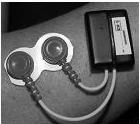
\includegraphics[height=0.16\textheight]{figs/Electrode} &
%    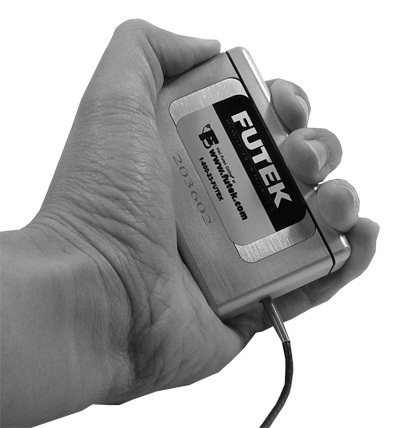
\includegraphics[height=0.16\textheight]{figs/Hand_Gripper} &
%    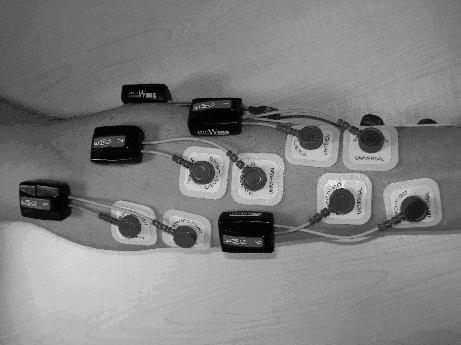
\includegraphics[height=0.16\textheight]{figs/El_Arrangement} \\
%    $(a)$ & $(b)$ & $(c)$ \\
%  \end{tabular}
%  \caption{The experimental setup (\textit{subject side}): $(a)$ an EMG
%    wireless electrode; $(b)$ the FUTEK force sensor; $(c)$ the typical
%    placement of the EMG electrodes on a subject's forearm (ventral side).}
%  \label{fig:SubjSetup}
%\end{figure*}

We employed the electrodes Aurion ZeroWire wireless EMG electrodes
%electrodes (see 
\cite{zerowire}. 
%The use of wireless electrodes helped the subjects
%freely move, to mimic their Daily-Life Activities (DLAs) during the
%acquisition.
%, not beeing wrapped in a thick net of electric cables. 
Moreover the subjects were given a FUTEK LMD500 Hand Gripper force
sensor \cite{LMD500} in order to measure the force applied by her/his
hand during the recording.

%Figure \ref{fig:SubjSetup} shows $(a)$ a single electrode, glued to the subject's forearm skin; $(b)$ the force sensor as gripped during a power grasp; and $(c)$ the typical placement of the electrodes (ventral side of the forearm).

We used a standard National Instruments data acquisition board
(NI-USB6211) connected to the receiver of the EMG wireless device and
to the force sensor, in order to record the sensors' signals and the
exerted force. We set the sampling rate of the board at $2$kHz, since
it is known that the raw EMG relevant bandwidth lies between $15$ and
$500$Hz. See Figure \ref{fig:spectra} for an example.
% To avoid synchronisation problems, we chose to record also
% the signal coming from the Hand Gripper at same sampling rate.

%The board was connected via a USB port to a custom National Instruments' LabView VI application (running on an entry-level laptop) to acquire all the signals.

\subsection{Data acquisition and pre-processing}
\label{sec:preproc}

%First of all we decided to record a rest condition to define the baseline of the EMG activity, than we started the experiment. 
We first considered a rest condition, so to define the baseline of the
EMG activity. We then proceded with the data recording:  
%It consisted
%of two phases, one right after the other:
%
%\begin{itemize}
%
%  \item Phase $1$: 
the subject kept her/his arm still and relaxed on a
    table, and was asked to grasp the force sensor using, in turn,
    three different grips (Figure~\ref{fig:Grasps}).
%
%  \item Phase $2$: the subject was asked to grasp the force sensor (as
%    she/he did in the previous phase) while freely moving, walking
%    around, lifting and pronating/supinating the arm and forearm,
%    sitting down and standing up from a chair. This should emulate the
%    main movements that one is expected to do during DLAs.
%
%\end{itemize}
%
%From now on, the two phases will be referred to as \emph{Still-Arm
%phase (SA)} and \emph{Free-Arm phase (FA)} respectively.

\begin{figure*}[!ht] \centering
  \begin{tabular}{ccc}
   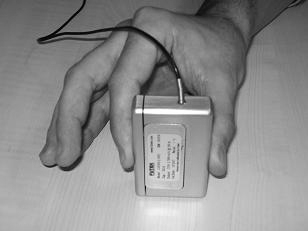
\includegraphics[height=0.16\textheight]{figs/grip1} &
    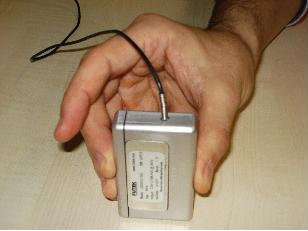
\includegraphics[height=0.16\textheight]{figs/grip2} &
    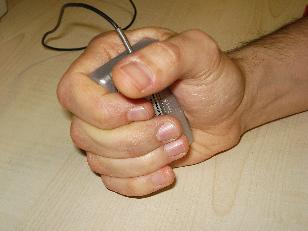
\includegraphics[height=0.16\textheight]{figs/grip3} \\
    $(a)$ & $(b)$ & $(c)$ \\
  \end{tabular}
  \caption{The three different grips employed in the experiment: $(a)$
   index precision grip; $(b)$ other fingers precision grip; $(c)$
   power grasp.}
  \label{fig:Grasps}
\end{figure*}

\begin{figure*}[!ht] \centering
  \begin{tabular}{cc}
    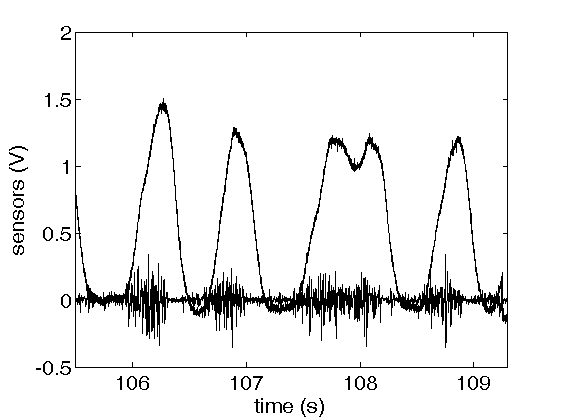
\includegraphics[width=0.45\textwidth]{figs/force_raw} &
    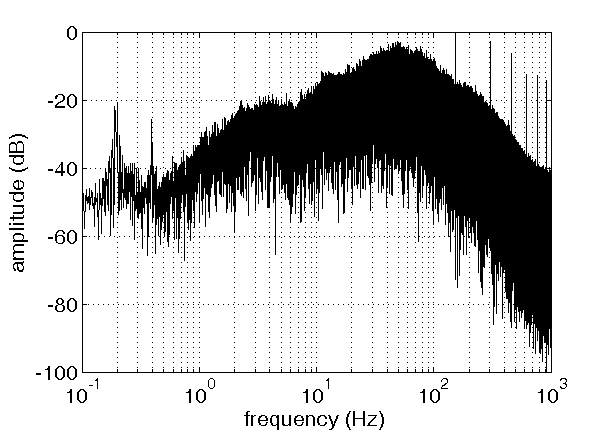
\includegraphics[width=0.45\textwidth]{figs/spectrum_raw} \\
    $(a)$ & $(b)$ \\
  \end{tabular}
  \caption{$(a)$ typical raw EMG and force signals; $(b)$ frequency diagram of
    the EMG signal.}
  \label{fig:spectra}
\end{figure*}

%During each phase,
The subject freely repeated each grasping action
for $100$'', resting for $30$'' in between grasps. In order to gather
more data and diminish the effect of local errors, the whole procedure
was repeated twice. As a whole, each subject's recording resulted in
about $2.4\times 10^6$ samples. 
%equally distributed in each phase.

Unlike commercial EMG electrodes, such as, e.g., Otto Bock's MyoBock
electrodes \cite{ottobock} that return the on-board computed Root-Mean
Square (RMS) of the EMG signal, the electrodes employed here return
the ``raw'' EMG signal.% within 10Hz and 1kHz.
%without any low-pass filtering or Root-Mean Square (RMS) processing.
Nevertheless, it is well-known \cite{deluca,zecca} that the force
exerted by a muscle is strongly related to the RMS of the EMG signal,
rather than to the raw signal. For this reason, in order to have a
signal that is as similar as possible to a \emph{control signal}, we
decided to evaluate the RMS, electrode by electrode.

For a given mono-variate discrete time-varying signal, the RMS is
defined as the mean of the squares of the signal values, evaluated
over a certain time-window $T_{RMS}$. Roughly speaking, the RMS acts
like an envelope extraction plus a low-pass filter, whose cutoff
frequency grows smaller as the time-window grows larger (i.e., as
$T_{RMS}$ becomes higher). For this reason, high values of $T_{RMS}$
imply an ostensible delay in the resulting signal that is due to
\emph{responsiveness} of the synthesized output signal.  It becomes
slower and slower as the $T_{RMS}$ value increases, since more
``samples'' are averaged to obtain a significant value. The choice of
$T_{RMS}$ is therefore crucial to produce a signal which is maximally
related to the force signal, unaffected by high-frequency noise, and
with an acceptable lag. However, it must be noted here that the EMG
signal, being directly related to the muscle \emph{activation
potentials}, happens to \emph{anticipate} the muscle
movements\footnote{The electromechanical delay (EMD) of a muscle is
defined as the interval between the onset of the electrical activity
of the muscle (EMG) indicating its activation by the neural system and
the onset of the resulting change in the mechanical variable
observed. The delays reported range from 25 to 100ms for different
muscles and tasks \cite{Wolf1994}.}. Therefore, in practical
applications, it can be considered as acceptable a wider lag than what
one would expect.
%a wider lag is acceptable than one would expect. 
This is useful since it allows us to increase $T_{RMS}$, if necessary.

%\begin{figure*}[!ht] \centering
%  \begin{tabular}{ccc}
%    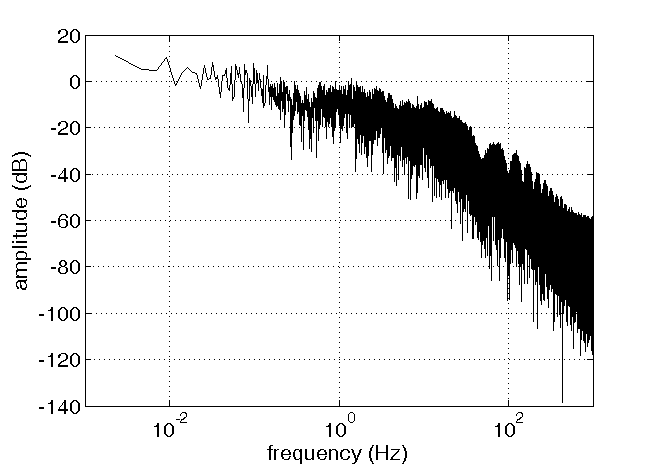
\includegraphics[width=0.3\textwidth]{figs/spectrum_RMS0040} &
%    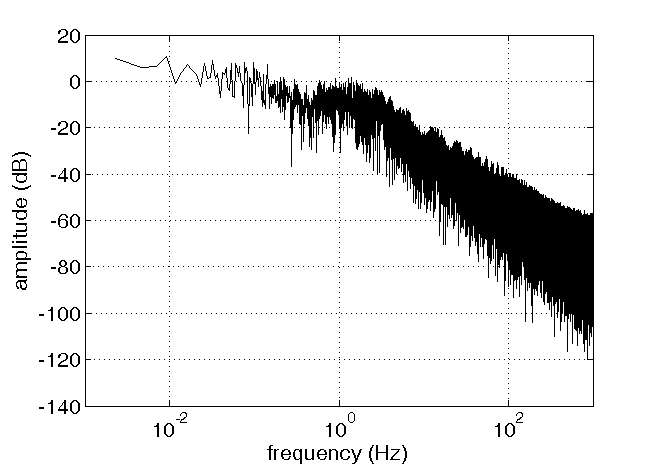
\includegraphics[width=0.3\textwidth]{figs/spectrum_RMS0200} &
%    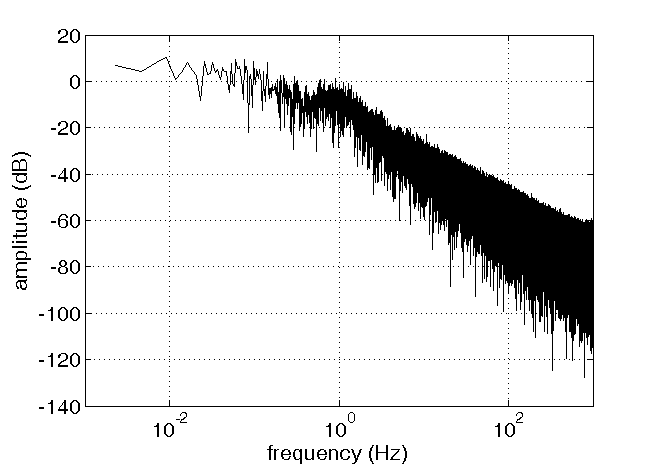
\includegraphics[width=0.3\textwidth]{figs/spectrum_RMS1000} \\
%    $(a)$ & $(b)$ & $(c)$ \\
%  \end{tabular}
%  \caption{(left to right) effects of the RMS on the bandwidth of the EMG
%    signals, for $T_{RMS} = 20, 100, 500ms$.}
%  \label{fig:RMSs}
%\end{figure*}

%Unfortunately 
We are not aware of any systematic way of setting a good value of
$T_{RMS}$ in such a framework. Therefore we found $T_{RMS}$
heuristically, according to some initial experiments.
% As an example, though, consider Figures \ref{fig:spectra} and \ref{fig:RMSs}.

Figure \ref{fig:spectra} (panel $(a)$) shows a few seconds of typical
force/EMG behaviour: it is apparent that the EMG signal starts oscillating when the force signal
starts increasing. It is also quite clear that the
amplitude of the envelope of the EMG is related to the force, as
indicated in the literature. Panel $(b)$ shows the frequency analysis
of the same EMG signal: as one can see, the meaningful bandwidth lies
in the interval known from the literature.

%On the other hand, Figure \ref{fig:RMSs} shows the effect of the RMS on the frequency components of the EMG, for three different values of $T_{RMS}$.
%It is clear that the meaningful bandwidth now contains all low-frequency components, possibly down to the constant, and is upper-bounded by about $25$Hz (panel $(a)$, for $T_{RMS}=20ms$) to $10$Hz (panel $(c)$, for $T_{RMS}=0.5s$). As expected, larger values of $T_{RMS}$ correspond to a better filtering but also to a larger delay.

This enables us to safely sub-sample the EMG signal after having
applied the RMS. Assuming that $T_{RMS}$ is not too small, we
subsampled both the EMG and force signal at $25$Hz, taking one sample
every $80$ of the original sequence.  This considerably reduced the
amount of data to be processed, namely to about $30.000$ samples for
each subject.

As a last data pre-processing step, we removed from the sample set
those samples for which the applied force was lower than a specific
threshold, in order to get a clearer representation of the activation
potentials. This threshold was chosen in order to remove a minimal
fraction of the samples. Of course, we fully retained the samples
corresponding to the baseline rest condition.  This is why we chose to
record this condition before the data acquisition.
%rest of the experiment.
